\documentclass[11pt,a4paper]{article}
\usepackage[utf8]{inputenc}
\usepackage[T1]{fontenc}
\usepackage[margin=1in]{geometry}
\usepackage{graphicx}
\usepackage{hyperref}
\usepackage{xcolor}
\usepackage{float}
\usepackage{listings}
\usepackage{upquote}
\usepackage{amsmath}
\usepackage{booktabs}

% Code listing style
\lstset{
    basicstyle=\ttfamily\small,
    breaklines=true,
    breakatwhitespace=false,
    frame=single,
    numbers=left,
    numberstyle=\tiny,
    backgroundcolor=\color{gray!10},
    keywordstyle=\color{blue},
    commentstyle=\color{green!50!black},
    stringstyle=\color{red},
    showstringspaces=false
}

\title{\textbf{LiDAR Sensing and Object Control in the Stretch Simulator}}
\author{
    Robotics and Cyber-Physical Systems \\
    School of Sciences and Engineering \\
    Tecnol\'ogico de Monterrey
}
\date{}

\begin{document}

\maketitle

\section*{Overview}

This document introduces two capabilities of the \texttt{stretch\_toolkit} simulator: reading and visualising LiDAR data, and manipulating free-floating objects in the scene at runtime. It also explains how to extend the default scene with real-world 3D-scanned objects sourced from a public dataset.

Both features are demonstrated through ready-to-run scripts (\texttt{lidar\_demo.py} and \texttt{object\_control\_demo.py}) that follow the same boilerplate structure used throughout the course.

% ─────────────────────────────────────────────────────────────────────────────
\newpage
\section{LiDAR Demo}

\subsection{What the Demo Does}

The Stretch robot model includes a simulated 2D LiDAR sensor mounted on the base. It produces 360 range measurements per scan—one per degree—each reporting the distance to the nearest obstacle in that direction. \texttt{lidar\_demo.py} reads these measurements every frame, drives the robot with the teleop provider, and renders a live top-down occupancy map in a separate window.

Run the demo with:

\begin{lstlisting}[language=bash]
uv run lidar_demo.py
\end{lstlisting}

Press \texttt{Q} or \texttt{Escape} in the visualisation window to quit.

\begin{figure}[H]
    \centering
    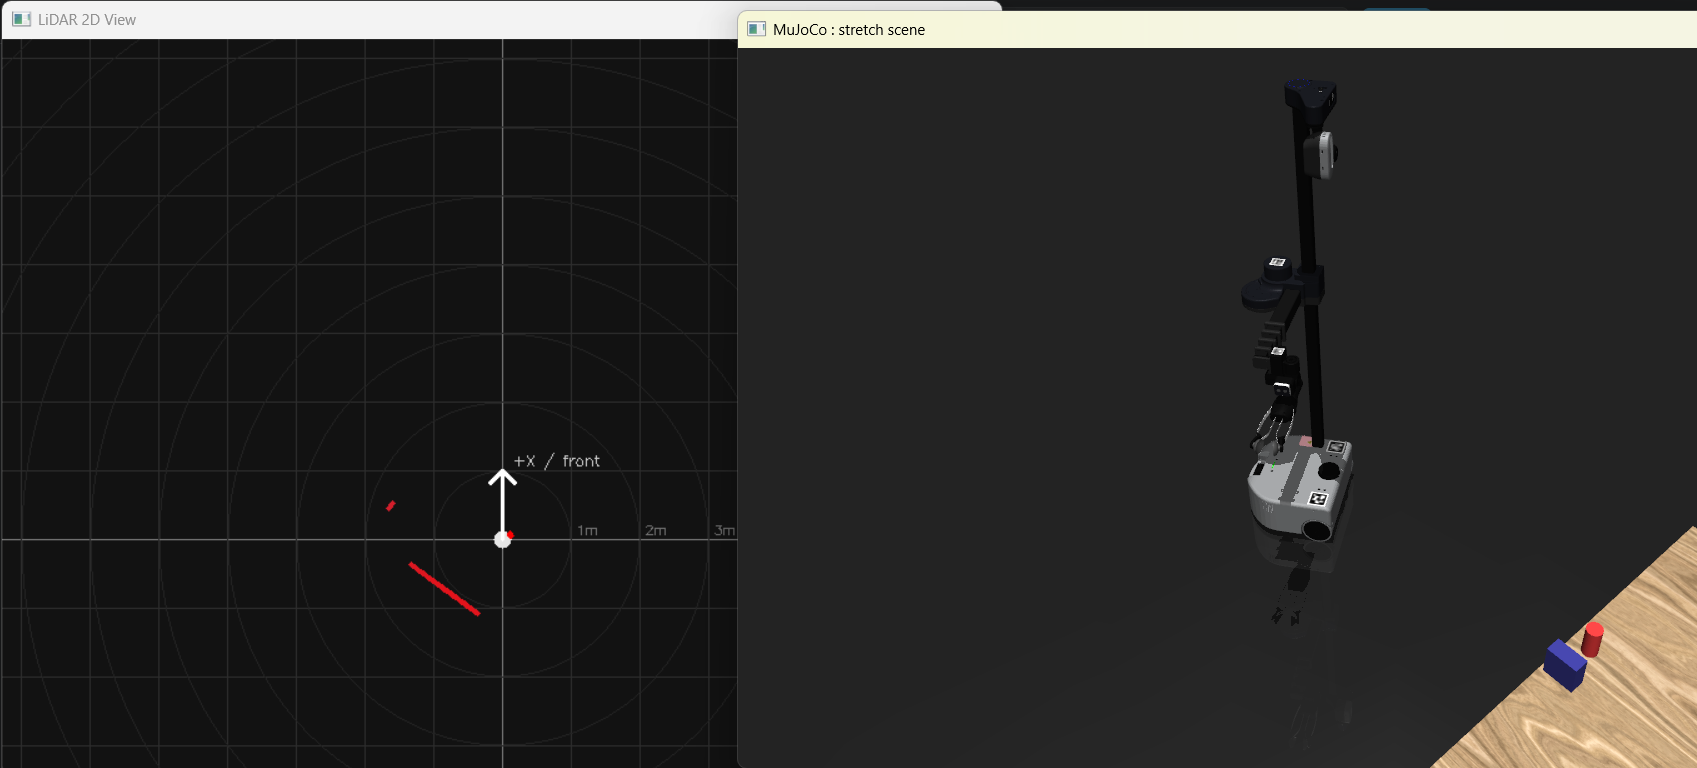
\includegraphics[width=0.75\textwidth]{lidar_demo.png}
    \caption{LiDAR demo: top-down 2D occupancy map rendered in real time. The robot is at the centre; detected obstacles appear as white dots.}
    \label{fig:lidar_demo}
\end{figure}

\subsection{How It Works}

The complete source is shown below.

\begin{lstlisting}[language=Python]
from stretch_toolkit import controller, BACKEND_NAME, LidarPlotter, TeleopProvider
import time

def main():
    print(f"\n=== Running on {BACKEND_NAME} backend ===\n")
    print("Displaying LiDAR scan. Press Q or Escape to quit.\n")

    plotter = LidarPlotter()
    tp = TeleopProvider(is_stretch_env=False)
    while True:
        ranges = controller.get_lidar_ranges()
        velocities = tp.get_normalized_velocities()
        controller.set_velocities(velocities)
        plotter.update(ranges)

        if plotter.should_quit():
            break

    plotter.close()

if __name__ == '__main__':
    main()
\end{lstlisting}

\paragraph{Key API calls}

\begin{itemize}
    \item \texttt{controller.get\_lidar\_ranges()} --- returns a 360-element \texttt{numpy} array of distances in metres. Rays that did not hit any geometry contain \texttt{numpy.inf}.
    \item \texttt{LidarPlotter()} --- creates an OpenCV window. Its \texttt{update(ranges)} method redraws the map each frame. Rays are drawn outward from the centre; shorter rays (closer obstacles) produce points nearer to the origin.
    \item \texttt{plotter.should\_quit()} --- returns \texttt{True} if the user pressed \texttt{Q} or \texttt{Escape} in the OpenCV window. Without this call the window would not respond to key presses.
    \item \texttt{plotter.close()} --- destroys the OpenCV window cleanly.
\end{itemize}

\paragraph{Backend transparency}

\texttt{controller.get\_lidar\_ranges()} is defined on the base \texttt{JointController} class. On the physical robot it reads from the actual sensor; in simulation it samples the MuJoCo ray-cast sensor. The rest of the demo code is identical for both backends.

% ─────────────────────────────────────────────────────────────────────────────
\newpage
\section{Object Control Demo}

\subsection{What the Demo Does}

The simulator scene contains bodies declared with a \texttt{<freejoint/>} in the scene XML. These bodies are not attached to the robot or any fixture---they can be moved freely in six degrees of freedom at runtime. \texttt{object\_control\_demo.py} enumerates all such bodies, lets the user cycle through them with the keyboard or gamepad, and moves the selected body using a second input layer.

Run the demo with:

\begin{lstlisting}[language=bash]
uv run object_control_demo.py
\end{lstlisting}

Press \texttt{Ctrl+C} in the terminal to quit.

\begin{figure}[H]
    \centering
    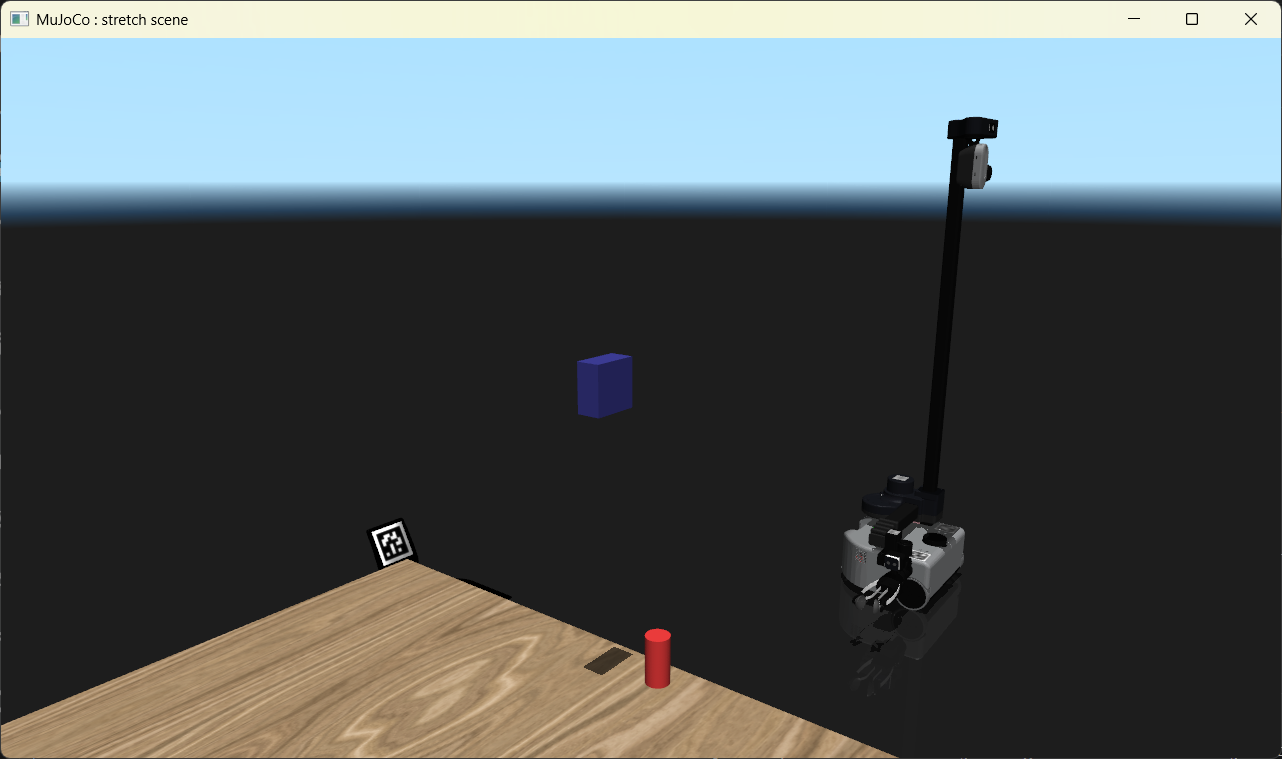
\includegraphics[width=0.75\textwidth]{object_control_demo.png}
    \caption{Object control demo: the selected object (highlighted in the MuJoCo viewer) is moved interactively. The terminal prints the current pose whenever the selection changes.}
    \label{fig:object_control_demo}
\end{figure}

\subsection{Controls}

The demo has two modes: \textbf{Object} (default) and \textbf{Teleop}. Press \texttt{Tab} or the gamepad \texttt{START} button to switch between them. The current mode is printed in the terminal whenever it changes.

\begin{center}
\begin{tabular}{lll}
\toprule
\textbf{Key / Button} & \textbf{Mode} & \textbf{Action} \\
\midrule
\texttt{t} / START      & Both   & Toggle Teleop $\leftrightarrow$ Object mode \\
\midrule
\texttt{m} / RB         & Object & Select next object \\
\texttt{n} / LB         & Object & Select previous object \\
\midrule
\texttt{z} / DPAD\,UP   & Object & Move up (+z) \\
\texttt{x} / DPAD\,DOWN & Object & Move down ($-$z) \\
\texttt{w} / \texttt{s} & Object & Move forward / backward (+y / $-$y) \\
\texttt{a} / \texttt{d} & Object & Move left / right ($-$x / +x) \\
\midrule
\texttt{i} / \texttt{k} & Object & Pitch + / $-$ \\
\texttt{j} / \texttt{l} & Object & Yaw + / $-$ \\
\texttt{u} / \texttt{o} & Object & Roll + / $-$ \\
\midrule
\texttt{g} / Y          & Object & Gravity \textbf{OFF} --- object floats \\
\texttt{f} / B          & Object & Gravity \textbf{ON}  --- object falls \\
\midrule
Standard teleop keys    & Teleop & Drive the robot base \\
\bottomrule
\end{tabular}
\end{center}

\subsection{How It Works}

\begin{lstlisting}[language=Python]
from stretch_toolkit import controller, BACKEND_NAME, ObjectControlProvider, TeleopProvider
import stretch_toolkit.input as inp
import time

MOVE_STEP = 0.02   # metres per tick
ROT_STEP  = 0.05   # radians per tick (~3 deg)
obj_ctrl  = ObjectControlProvider(move_step=MOVE_STEP, rot_step=ROT_STEP)
tp        = TeleopProvider(is_stretch_env=False)

def main():
    objects = controller.list_scene_objects()
    selected = 0
    mode = "object"

    while True:
        # --- Toggle mode (Tab on keyboard, START on gamepad) --------
        if inp.rising_edge("t", "START"):
            mode = "teleop" if mode == "object" else "object"
            print(f"[Mode: {mode}]")
            if mode == "object":
                controller.set_velocities({"base_forward": 0,
                                           "base_counterclockwise": 0})

        if mode == "teleop":
            velocities = tp.get_normalized_velocities()
            controller.set_velocities(velocities)
        else:
            prev = selected
            selected = (selected
                        + inp.rising_edge("RB", "m")
                        - inp.rising_edge("LB", "n")) % len(objects)

            if selected != prev:
                print(f"Selected: {objects[selected]}")
                pose = controller.get_object_pose(objects[selected])
                if pose:
                    print(f"  x={pose['x']:.3f}  y={pose['y']:.3f}  z={pose['z']:.3f}  "
                          f"qw={pose['qw']:.3f}  qx={pose['qx']:.3f}  "
                          f"qy={pose['qy']:.3f}  qz={pose['qz']:.3f}")

            delta, gravity = obj_ctrl.get_delta()
            controller.move_object_by(objects[selected], delta)
            controller.set_object_gravity(objects[selected], gravity)

        time.sleep(1 / 30)
\end{lstlisting}

\paragraph{Key API calls}

\begin{itemize}
    \item \texttt{controller.list\_scene\_objects()} --- parses the active scene XML and returns the names of every body that contains a \texttt{<freejoint/>}. The list is computed once at startup; it works identically whether you are using the default scene or a RoboCasa kitchen.

    \item \texttt{inp.rising\_edge("t", "START")} --- detects the \texttt{t} key or the gamepad Start button to toggle modes. Tab was deliberately avoided as MuJoCo reserves it for its own viewer shortcuts.

    \item \texttt{inp.rising\_edge("RB", "m")} --- returns \texttt{True} (coerced to \texttt{1}) exactly once when either the gamepad \texttt{RB} button or the keyboard \texttt{m} key is first pressed. The multi-argument form checks any of the supplied inputs. Subtracting a second \texttt{rising\_edge} call gives $+1$, $-1$, or $0$ in a single expression, which is used here to advance or retreat the selection index.

    \item \texttt{ObjectControlProvider.get\_delta()} --- samples all movement and rotation keys and returns a pair \texttt{(delta, gravity)} where \texttt{delta} is a dict of axis offsets (only non-zero axes are included) and \texttt{gravity} is \texttt{True}, \texttt{False}, or \texttt{None} (no change this frame).

    \item \texttt{controller.move\_object\_by(name, delta)} --- applies the delta dict to the named freejoint body. An empty dict is silently ignored, so no guard is needed in the loop.

    \item \texttt{controller.set\_object\_gravity(name, gravity)} --- sets gravity compensation for the body: \texttt{False} makes it float, \texttt{True} makes it fall. \texttt{None} is a no-op.

    \item \texttt{controller.get\_object\_pose(name)} --- returns the current world pose as a dict with keys \texttt{x}, \texttt{y}, \texttt{z}, \texttt{qw}, \texttt{qx}, \texttt{qy}, \texttt{qz}. The pose is printed whenever the selection changes so that you can copy the coordinates directly into \texttt{scene.xml} to set a new default start position.
\end{itemize}

\paragraph{Pose printing for scene configuration}

Whenever you cycle to a different object the terminal prints its current world pose:

\begin{lstlisting}[language=bash]
Selected: android_lego
  x=0.180  y=-0.550  z=0.821  qw=0.999  qx=0.000  qy=0.032  qz=0.000
\end{lstlisting}

You can use these values directly as the \texttt{pos} and \texttt{quat} attributes of the body in \texttt{scene.xml} to save a preferred start configuration.

% ─────────────────────────────────────────────────────────────────────────────
\newpage
\section{Adding Custom 3D-Scanned Objects}

\subsection{The MuJoCo Scanned Objects Dataset}

The \href{https://github.com/kevinzakka/mujoco_scanned_objects}{mujoco\_scanned\_objects} repository by Kevin Zakka contains roughly 1\,000 real-world objects captured with photogrammetry. Every object folder provides:

\begin{itemize}
    \item \texttt{model.obj} --- the textured 3D mesh (Wavefront OBJ format)
    \item \texttt{texture.png} --- the colour texture image
    \item \texttt{model.xml} --- a standalone MuJoCo XML fragment showing how the asset is typically loaded, including pre-computed V-HACD collision decomposition meshes (\texttt{model\_collision\_*.obj})
    \item \texttt{model\_collision\_*.obj} --- fine-grained collision meshes (optional; a single box is sufficient for most use cases)
\end{itemize}

\begin{figure}[H]
    \centering
    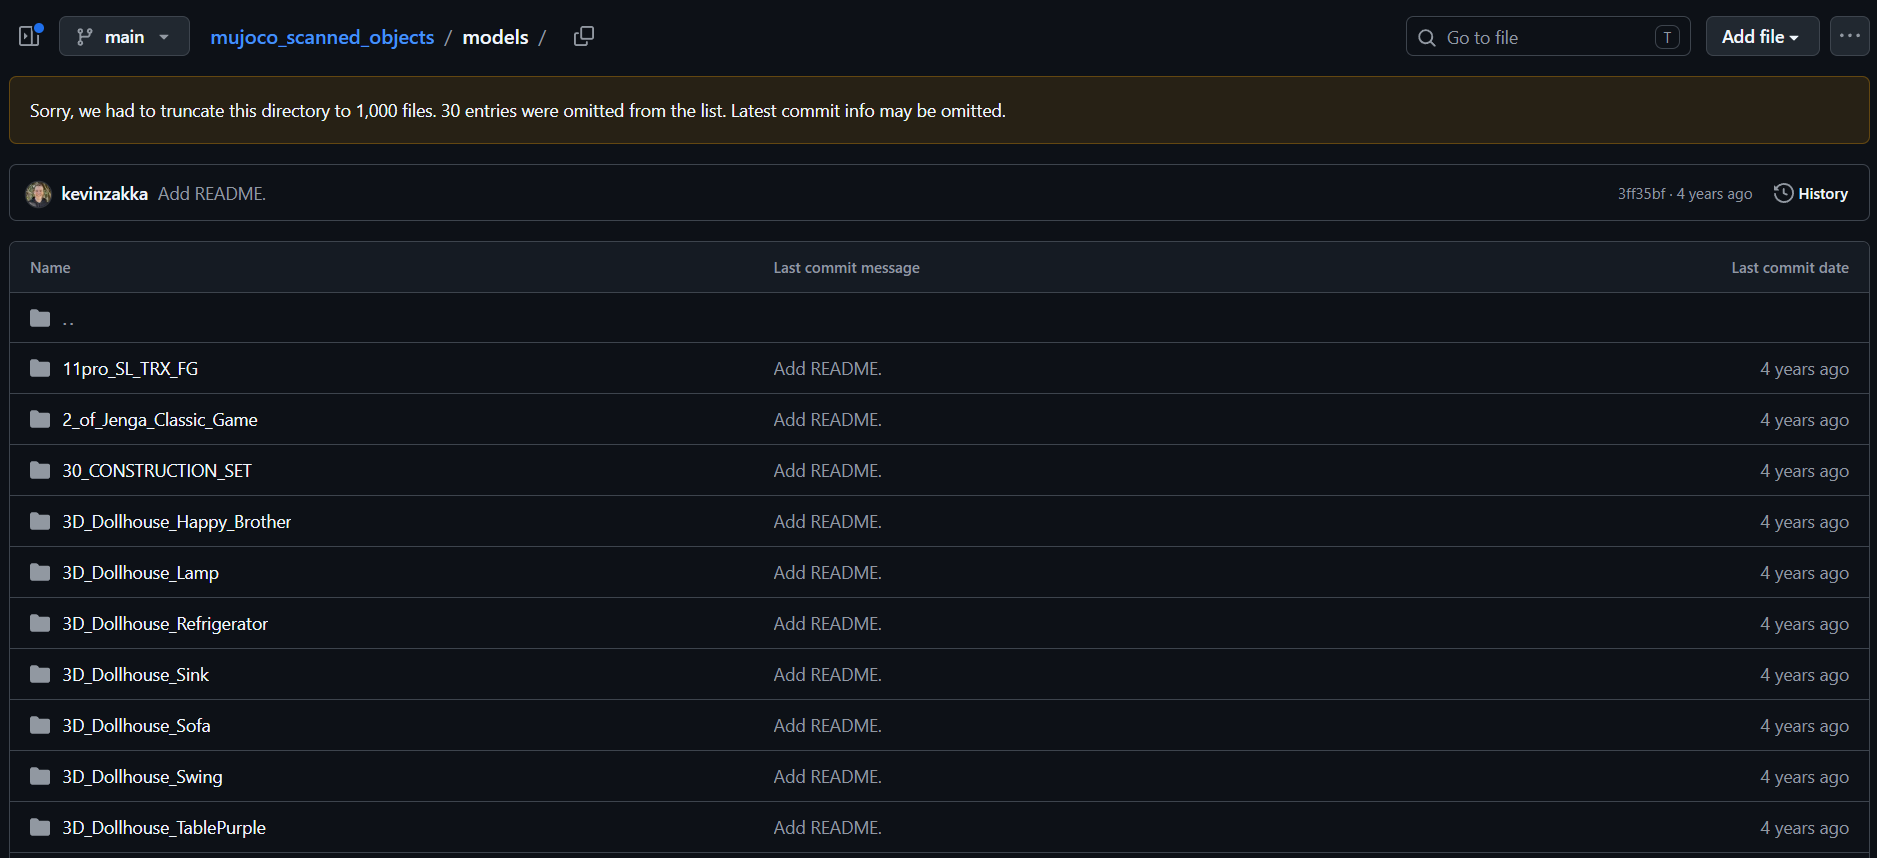
\includegraphics[width=0.75\textwidth]{mujoco_scanned_objects.png}
    \caption{A selection of objects from the mujoco\_scanned\_objects dataset. Each row corresponds to one folder in the \texttt{models/} directory.}
    \label{fig:mso_overview}
\end{figure}

\subsection{Asset Placement}

Assets must be placed under:

\begin{lstlisting}
stretch_mujoco/models/assets/custom_objects/mujoco_scanned_objects/models/<ObjectName>/
\end{lstlisting}

\texttt{stretch.xml} sets \texttt{assetdir="assets"}, so paths inside \texttt{scene.xml} are resolved relative to that directory automatically. Only two files are required from each object folder: \texttt{model.obj} and \texttt{texture.png}.

\subsection{Downloading Assets}

\paragraph{Concrete example --- Android Lego figure}

\begin{lstlisting}[language=bash]
$base = "https://raw.githubusercontent.com/kevinzakka/mujoco_scanned_objects/main/models/Android_Lego"
$dest = "stretch_mujoco/models/assets/custom_objects/mujoco_scanned_objects/models/Android_Lego"
New-Item -ItemType Directory -Force -Path $dest
Invoke-WebRequest "$base/model.obj"   -OutFile "$dest/model.obj"
Invoke-WebRequest "$base/texture.png" -OutFile "$dest/texture.png"
\end{lstlisting}

\paragraph{Template for any other object}

Replace \texttt{<ObjectName>} with the exact folder name from the repository (case-sensitive):

\begin{lstlisting}[language=bash]
$obj  = "<ObjectName>"
$base = "https://raw.githubusercontent.com/kevinzakka/mujoco_scanned_objects/main/models/$obj"
$dest = "stretch_mujoco/models/assets/custom_objects/mujoco_scanned_objects/models/$obj"
New-Item -ItemType Directory -Force -Path $dest
Invoke-WebRequest "$base/model.obj"   -OutFile "$dest/model.obj"
Invoke-WebRequest "$base/texture.png" -OutFile "$dest/texture.png"
\end{lstlisting}

You can browse available object names at:
\url{https://github.com/kevinzakka/mujoco_scanned_objects/tree/main/models}

\subsection{Adding the Object to \texttt{scene.xml}}

Once the files are in place, edit \texttt{stretch\_mujoco/models/scene.xml} to declare the assets and add a freejoint body. The structure below is the canonical pattern used for the Android Lego figure.

\begin{lstlisting}[language=XML]
<!-- Inside <asset> -->
<texture name="android_lego_texture" type="2d"
         file="custom_objects/mujoco_scanned_objects/models/Android_Lego/texture.png"/>
<material name="android_lego_material" texture="android_lego_texture"/>
<mesh name="android_lego_mesh"
      file="custom_objects/mujoco_scanned_objects/models/Android_Lego/model.obj"
      scale="1 1 1"/>

<!-- Inside <worldbody> -->
<body name="android_lego" pos="0.18 -0.55 0.75" gravcomp="1">
  <freejoint/>

  <!-- Visual mesh only (no collision contribution) -->
  <geom name="android_lego_visual" type="mesh"
        mesh="android_lego_mesh" material="android_lego_material"
        contype="0" conaffinity="0" density="0"/>

  <!-- Invisible collision approximation -->
  <geom name="android_lego_collision" type="box"
        pos="0 0 0.045" size="0.028 0.020 0.042"
        mass="0.10" rgba="1 0 0 0" friction="1 0.005 0.0001"/>
</body>
\end{lstlisting}

\paragraph{Why two geoms?}

MuJoCo can use any mesh for collision, but fine-grained mesh collision is computationally expensive and can cause instability. The recommended pattern is to keep the visual mesh display-only (\texttt{contype="0" conaffinity="0" density="0"}) and add a separate primitive geom (box, cylinder, or sphere) as the physics proxy. Set \texttt{rgba="... 0"} on the collision geom to keep it invisible in the viewer and camera feeds.

\paragraph{Collision size}

The \texttt{model.xml} file inside each object folder, while not used directly, gives you the object's bounding information. Use the object control demo (\S\,2) to move the object around after adding it---if the collision proxy is obviously wrong (the object sinks through the table or floats above it), adjust the \texttt{size} and \texttt{pos} values of the collision geom.

\paragraph{\texttt{gravcomp="1"}}

Setting \texttt{gravcomp="1"} on the body makes it start in a floating state (gravity fully compensated). This is consistent with the \texttt{set\_object\_gravity} API: calling it with \texttt{enabled=False} keeps the object floating, \texttt{enabled=True} lets it fall. The default in the demo is floating so that objects stay where you place them until gravity is explicitly enabled.

\paragraph{Freejoint and \texttt{list\_scene\_objects()}}

Any body with a \texttt{<freejoint/>} is automatically discovered by \texttt{controller.list\_scene\_objects()} and immediately controllable via the object control demo without any additional code changes.

\begin{figure}[H]
    \centering
    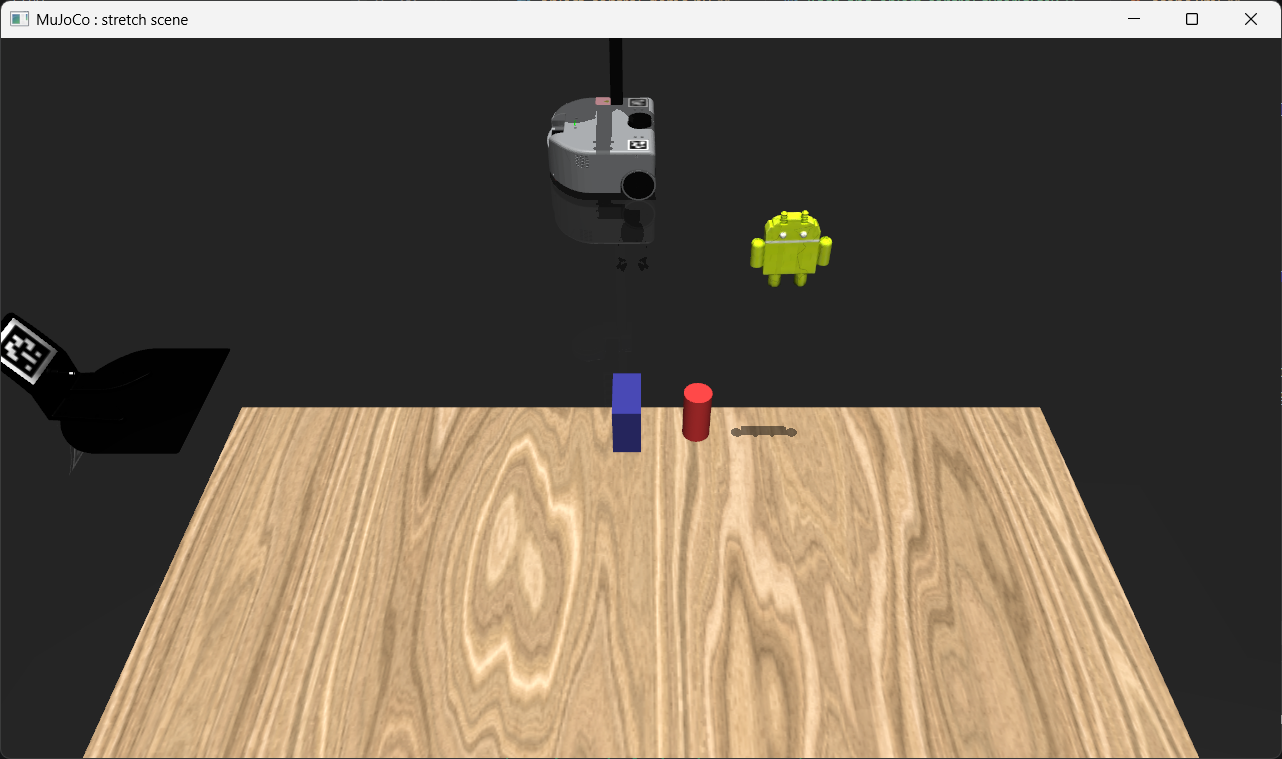
\includegraphics[width=0.75\textwidth]{android_lego_scene.png}
    \caption{The Android Lego figure placed on the table alongside the existing primitive objects. All three bodies are selectable and movable in the object control demo.}
    \label{fig:android_lego_scene}
\end{figure}

\subsection{Adding Objects to a RoboCasa Kitchen}

When the simulator is configured to use a RoboCasa kitchen environment (\texttt{robocasa.enabled: true} in \texttt{stretch\_toolkit/sim\_config.json}), the scene XML is generated procedurally at startup rather than loaded from a static file. Custom objects are injected into this generated XML through the \texttt{custom\_objects} array in the same config file.

\paragraph{Configuration}

Open \texttt{stretch\_toolkit/sim\_config.json} and add entries to the \texttt{custom\_objects} array inside the \texttt{robocasa} block:

\begin{lstlisting}[language={}]
{
  "robocasa": {
    "enabled": true,
    "task": "PnPCounterToCab",
    "layout": 0,
    "style": 0,
    "custom_objects": [
      {
        "name": "android_lego",
        "obj":  "custom_objects/mujoco_scanned_objects/models/Android_Lego/model.obj",
        "texture": "custom_objects/mujoco_scanned_objects/models/Android_Lego/texture.png",
        "pos": [0.0, 0.0, 1.0],
        "collision_size": [0.028, 0.020, 0.042],
        "collision_pos":  [0.0, 0.0, 0.045],
        "mass": 0.10,
        "gravcomp": 1.0
      }
    ]
  }
}
\end{lstlisting}

\paragraph{Config fields}

\begin{itemize}
    \item \texttt{name} --- the MuJoCo body name; must be unique within the scene. This is also the name returned by \texttt{list\_scene\_objects()} and accepted by \texttt{move\_object\_by} and \texttt{get\_object\_pose}.
    \item \texttt{obj} / \texttt{texture} --- paths relative to \texttt{stretch\_mujoco/models/assets/}. These must point to the same files downloaded in \S\,3.3.
    \item \texttt{pos} --- \texttt{[x, y, z]} world position in metres. Because the kitchen layout varies, \texttt{[0, 0, 1]} (one metre above the floor) is a safe starting value; adjust after viewing the scene.
    \item \texttt{collision\_size} / \texttt{collision\_pos} --- half-extents and local offset of the box collision proxy, in metres. Same meaning as the \texttt{size} / \texttt{pos} attributes in the \texttt{scene.xml} approach.
    \item \texttt{mass} --- body mass in kilograms.
    \item \texttt{gravcomp} --- \texttt{1.0} to start floating, \texttt{0.0} to start falling under gravity.
\end{itemize}

\paragraph{How injection works}

At startup \texttt{stretch\_toolkit} reads the config, calls \texttt{model\_generation\_wizard} to produce the kitchen XML string, and then calls \texttt{xml\_inject\_mesh\_object} once per entry to splice the asset declarations and freejoint body into the string before passing it to MuJoCo. No manual XML editing is required---only the JSON config entry and the two asset files on disk.

\begin{figure}[H]
    \centering
    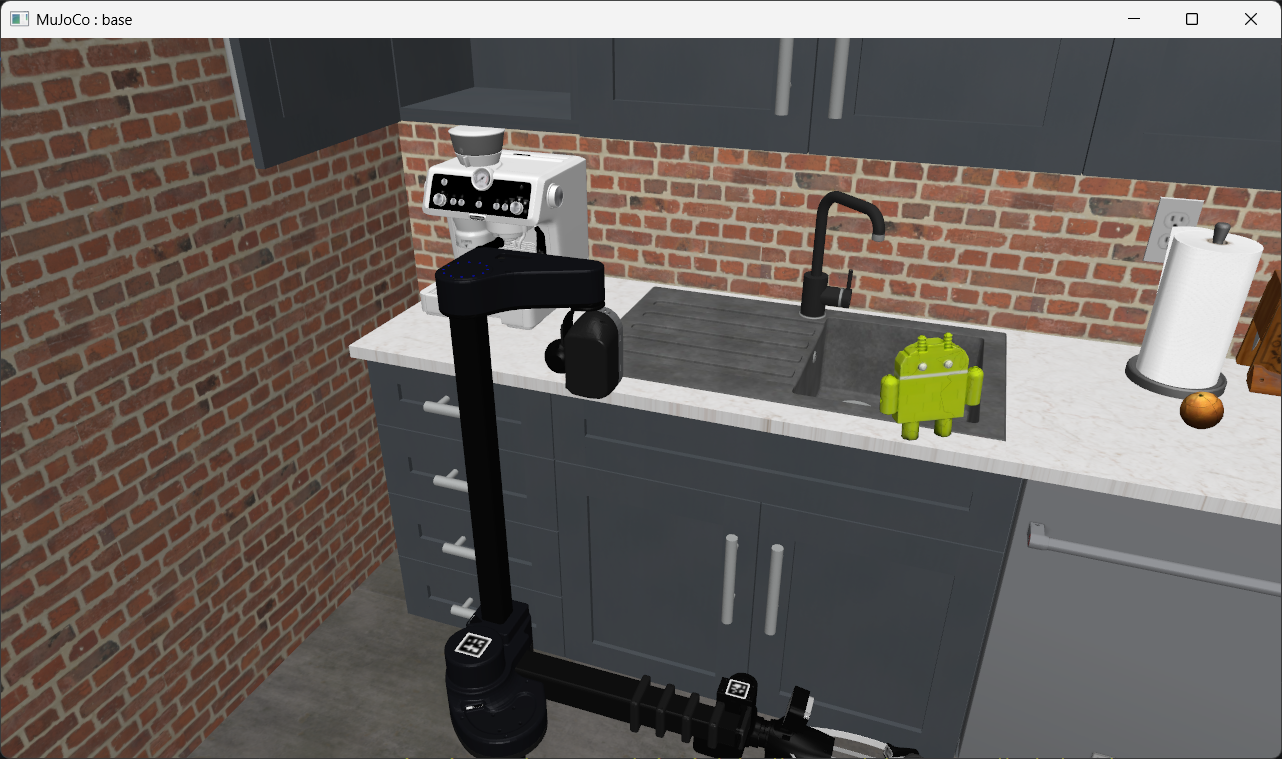
\includegraphics[width=0.75\textwidth]{robocasa_custom_object.png}
    \caption{The Android Lego figure spawned inside a RoboCasa kitchen via \texttt{sim\_config.json}. The object is immediately selectable in the object control demo.}
    \label{fig:robocasa_custom_object}
\end{figure}

\end{document}
